\documentclass{standalone}
\usepackage{tikz}
\usetikzlibrary{shapes}
\usetikzlibrary{positioning}
\usepackage{amsmath}


\begin{document}
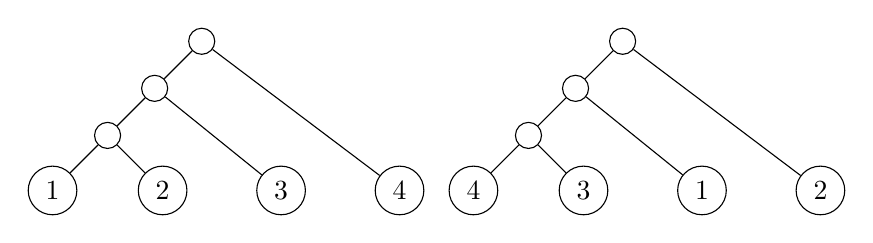
\begin{tikzpicture}[node distance=2cm]

    \node(A1)[draw, circle, minimum size=0.2cm]{};
    \node(B1)[draw, circle, minimum size=0.2cm, below left=0.5cm of A1]{};
    
    \node(D1)[draw, circle, minimum size=0.2cm, below left=0.5cm of B1]{};
    \node(F1)[draw, circle, minimum size=0.2cm, below left=0.5cm of D1]{1};
    \node(G1)[draw, circle, minimum size=0.2cm, below right=0.5cm of D1]{2};
    \node(E1)[draw, circle, minimum size=0.2cm, right=0.8727922cm of G1]{3};
    \node(C1)[draw, circle, minimum size=0.2cm, right=0.8727922cm of E1]{4};
    
    \draw (A1) -- (B1) -- (D1) -- (F1);
    \draw (D1) -- (G1);
    \draw (B1) -- (E1);
    \draw (A1) -- (C1);
    


    \node(A)[draw, circle, minimum size=0.2cm, right=5cm of A1]{};
    \node(B)[draw, circle, minimum size=0.2cm, below left=0.5cm of A]{};
    
    \node(D)[draw, circle, minimum size=0.2cm, below left=0.5cm of B]{};
    \node(F)[draw, circle, minimum size=0.2cm, below left=0.5cm of D]{4};
    \node(G)[draw, circle, minimum size=0.2cm, below right=0.5cm of D]{3};
    \node(E)[draw, circle, minimum size=0.2cm, right=0.8727922cm of G]{1};
    \node(C)[draw, circle, minimum size=0.2cm, right=0.8727922cm of E]{2};
    
    \draw (A) -- (B) -- (D) -- (F);
    \draw (D) -- (G);
    \draw (B) -- (E);
    \draw (A) -- (C);
    



\end{tikzpicture}
\end{document}
